\documentclass[journal,12pt,twocolumn]{IEEEtran}

\usepackage{setspace}
\usepackage{gensymb}
\singlespacing
\usepackage[cmex10]{amsmath}

\usepackage{amsthm}

\usepackage{mathrsfs}
\usepackage{txfonts}
\usepackage{amsmath}
\usepackage{stfloats}
\usepackage{float}
\usepackage{bm}
\usepackage{tikz}
\usepackage{pgfplots}
\pgfplotsset{compat=1.7}
\usepackage{cite}
\usepackage{cases}
\usepackage{subfig}

\usepackage{longtable}
\usepackage{multirow}

\usepackage{enumitem}
\usepackage{mathtools}
\usepackage{steinmetz}
\usepackage{tikz}
\usepackage{circuitikz}
\usepackage{verbatim}
\usepackage{tfrupee}
\usepackage[breaklinks=true]{hyperref}
\usepackage{graphicx}
\usepackage{tkz-euclide}

\usetikzlibrary{calc,math}
\usetikzlibrary{shapes.geometric, arrows}
\usepackage{listings}
    \usepackage{color}                                            %%
    \usepackage{array}                                            %%
    \usepackage{longtable}                                        %%
    \usepackage{calc}                                             %%
    \usepackage{multirow}                                         %%
    \usepackage{hhline}                                           %%
    \usepackage{ifthen}                                           %%
    \usepackage{lscape}
\usepackage{multicol}
\usepackage{chngcntr}
\usepackage{hyperref}
\hypersetup{
    colorlinks=true,
    linkcolor=blue,
    filecolor=blue,
    urlcolor=blue,
}
\DeclareMathOperator*{\Res}{Res}
\DeclareMathOperator{\sinc}{sinc}
\DeclareMathOperator{\Sa}{Sa}
\DeclareMathOperator{\rect}{rect}

\renewcommand\thesection{\arabic{section}}
\renewcommand\thesubsection{\thesection.\arabic{subsection}}
\renewcommand\thesubsubsection{\thesubsection.\arabic{subsubsection}}



\hyphenation{optical networks semiconduc-tor}
\def\inputGnumericTable{}                                 %%

\lstset{
%language=C,
frame=single, 
breaklines=true,
columns=fullflexible
}
\date{March 2021}

\makeatletter
\setlength{\@fptop}{0pt}
\makeatother

\begin{document}

\newtheorem{theorem}{Theorem}[section]
\newtheorem{problem}{Problem}
\newtheorem{proposition}{Proposition}[section]
\newtheorem{lemma}{Lemma}[section]
\newtheorem{corollary}[theorem]{Corollary}
\newtheorem{example}{Example}[section]
\newtheorem{definition}[problem]{Definition}

\newcommand{\BEQA}{\begin{eqnarray}}
\newcommand{\EEQA}{\end{eqnarray}}
\newcommand{\define}{\stackrel{\triangle}{=}}
\bibliographystyle{IEEEtran}
\raggedbottom
\setlength{\parindent}{0pt}
\providecommand{\mbf}{\mathbf}
\providecommand{\pr}[1]{\ensuremath{\Pr\left(#1\right)}}
\providecommand{\qfunc}[1]{\ensuremath{Q\left(#1\right)}}
\providecommand{\fn}[1]{\ensuremath{f\left({#1}\right)}}
\providecommand{\e}[1]{\ensuremath{E\left(#1\right)}}
\providecommand{\sbrak}[1]{\ensuremath{{}\left[#1\right]}}
\providecommand{\lsbrak}[1]{\ensuremath{{}\left[#1\right.}}
\providecommand{\rsbrak}[1]{\ensuremath{{}\left.#1\right]}}
\providecommand{\brak}[1]{\ensuremath{\left(#1\right)}}
\providecommand{\lbrak}[1]{\ensuremath{\left(#1\right.}}
\providecommand{\rbrak}[1]{\ensuremath{\left.#1\right)}}
\providecommand{\cbrak}[1]{\ensuremath{\left\{#1\right\}}}
\providecommand{\lcbrak}[1]{\ensuremath{\left\{#1\right.}}
\providecommand{\rcbrak}[1]{\ensuremath{\left.#1\right\}}}
\theoremstyle{remark}
\newtheorem{rem}{Remark}
\newcommand{\sgn}{\mathop{\mathrm{sgn}}}
\newcommand{\comb}[2]{{}^{#1}\mathrm{C}_{#2}}
\providecommand{\abs}[1]{\vert#1\vert}
\providecommand{\res}[1]{\Res\displaylimits_{#1}} 
\providecommand{\norm}[1]{\lVert#1\rVert}
%\providecommand{\norm}[1]{\lVert#1\rVert}
\providecommand{\mtx}[1]{\mathbf{#1}}
\providecommand{\mean}[1]{E\sbrak{ #1 }}
\providecommand{\fourier}{\overset{\mathcal{F}}{ \rightleftharpoons}}
%\providecommand{\hilbert}{\overset{\mathcal{H}}{ \rightleftharpoons}}
\providecommand{\system}{\overset{\mathcal{H}}{ \longleftrightarrow}}
	%\newcommand{\solution}[2]{\textbf{Solution:}{#1}}
\newcommand{\solution}{\noindent \textbf{Solution: }}
\newcommand{\cosec}{\,\text{cosec}\,}
\providecommand{\dec}[2]{\ensuremath{\overset{#1}{\underset{#2}{\gtrless}}}}
\newcommand{\myvec}[1]{\ensuremath{\begin{pmatrix}#1\end{pmatrix}}}
\newcommand{\mydet}[1]{\ensuremath{\begin{vmatrix}#1\end{vmatrix}}}
\numberwithin{equation}{subsection}
\makeatletter
\@addtoreset{figure}{problem}
\makeatother
\let\StandardTheFigure\thefigure
\let\vec\mathbf

\vspace{3cm}
\title{EE3900 Gate Assignment - 4}
\author{Adhvik Mani Sai Murarisetty - AI20BTECH11015}
\maketitle
\newpage
\bigskip
\renewcommand{\thetable}{\theenumi}

Download latex-tikz codes from 
%
\begin{lstlisting}
https://github.com/adhvik24/EE3900/blob/main/Gate_A4/main.tex
\end{lstlisting}
%
Download python codes from 
%
\begin{lstlisting}
https://github.com/adhvik24/EE3900/blob/main/Gate_A4/codes/plot.py
\end{lstlisting}
\section*{Problem}
(GATE EC-1997 Qn 5.2) If the fourier transform of the deterministic signal $x(t)$ is $X(f)$, then
\begin{enumerate}
    \item The fourier transform of $x(t-2)$ is
    \begin{enumerate} 
        \item $X(f)e^{-j4\pi f}$
        \item $X(2f)$
        \item $2X(2f)$
        \item $X(f-2)$
    \end{enumerate}
    \item The fourier transform of $x(\frac{t}{2})$ is
    \begin{enumerate} 
        \item $X(f)e^{-j4\pi f}$
        \item $X(2f)$
        \item $2X(2f)$
        \item $X(f-2)$
    \end{enumerate}
\end{enumerate}

\section*{Solution}
\begin{enumerate}
    
\item By the time shifting property of Fourier transform,
\begin{align}
    x(t - t_0)&\fourier{e^{-j2\pi ft_0}X(f)}\\
    x\brak{{t-2}}&\fourier {e^{-{j4\pi f}}X\brak{f}}
\end{align}


Let $x(t) = \rect{\brak{t}}$ and $\sinc(t) = \frac{\sin(t)}{t}$
\begin{align}
    X(f) = \sinc\brak{f}
\end{align}
For $x(t) = \rect{\brak{t-2}}$,
\begin{align}
    e^{-{j4\pi f}}X\brak{f} = e^{-{j4\pi f}}\sinc\brak{{f}}
\end{align}
The correct option is (a).
\begin{figure}
    \centering
    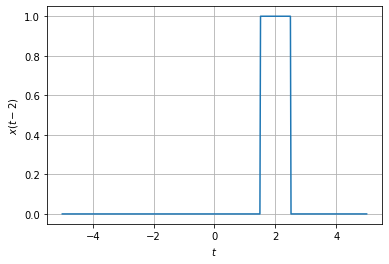
\includegraphics[width = \columnwidth]{t-21.png}
    \caption{Plot of rect(t-2)}
    \label{fig:my_label}
\end{figure}
\begin{figure}
    \centering
    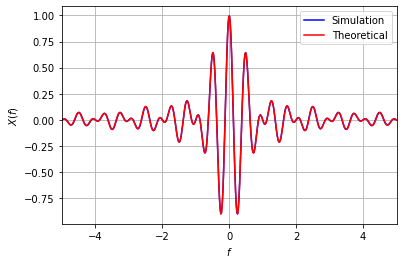
\includegraphics[width = \columnwidth]{t-22.png}
    \caption{Fourier transform Simulation v/s Theoretical}
    \label{fig:my_label1}
\end{figure}
\item By the time scaling property of Fourier transform,
\begin{align}
    x(\alpha t)&\fourier{\frac{1}{|\alpha|}}X\brak{\frac{f}{|\alpha|}}\\
    x(\frac{t}{2})&\fourier2X\brak{2f}
\end{align}
Let $x(t) = \rect{\brak{t}}$ and $\sinc(t) = \frac{\sin(t)}{t}$
\begin{align}
    X(f) = \sinc\brak{f}
\end{align}
For $x(t) = \rect{\brak{\frac{t}{2}}}$,
\begin{align}
    {2}X\brak{{2f}} = {2}\sinc\brak{{2f}}
\end{align}
The correct option is (c).
\begin{figure}
    \centering
    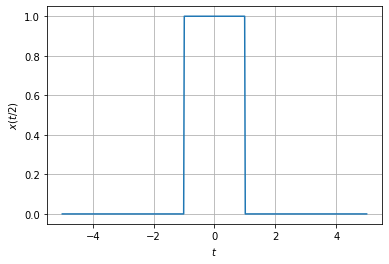
\includegraphics[width = \columnwidth]{t_21.png}
    \caption{Plot of rect($\frac{t}{2}$)}
    \label{fig:my_label2}
\end{figure}
\begin{figure}
    \centering
    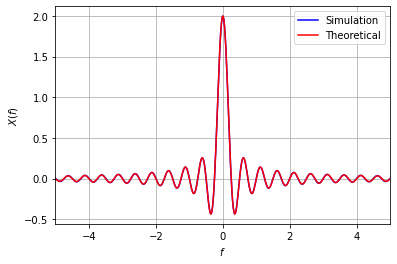
\includegraphics[width = \columnwidth]{t_22.png}
    \caption{Fourier transform Simulation v/s Theoretical}
    \label{fig:my_label3}
\end{figure}
\end{enumerate}


\end{document}
